\begin{figure*}[t]
  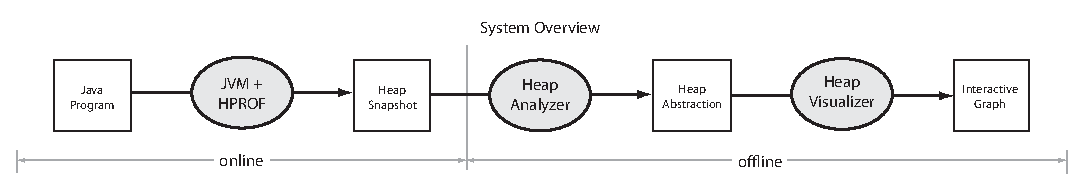
\includegraphics[width=\textwidth]{figs/system-flowchart}
  \caption{The Heapviz pipeline.  The JVM and HPROF generate a heap 
  snapshot from a running Java program.  Our heap analyzer then parses 
  this snapshot, builds a graph representation of the concrete heap, 
  summarizes the graph, and outputs a heap abstraction.  Our heap 
  visualizer reads the heap abstraction and displays the graph, enabling 
  the user to explore it interactively.  }
  \label{fig:pipeline}
\end{figure*}

\section{System Overview}

In this section, we provide a brief overview of the architecture of Heapviz.
We go into further detail in Sections~\ref{analysis} and~\ref{visualization}.
The full Heapviz pipeline (Figure~\ref{fig:pipeline}) consists of three major
parts:

\begin{enumerate}

\item \textbf{JVM + HPROF.} Generates a heap snapshot from a running Java
  program using the HPROF tool~\cite{hprof} provided by Sun with the Java
  Development Kit.

\item \textbf{Heap analyzer.} Parses the heap snapshot, builds a graph
  representation of the concrete heap, summarizes the graph, and outputs the
  resulting heap abstraction.

\item \textbf{Heap visualizer.} Reads the heap abstraction and displays the
  (possibly large) graph, allowing the user to explore it interactively.

\end{enumerate}

% SZG: this description is a little redundant with the bullet list above, but I think it's ok

Our \emph{heap analyzer} parses the heap snapshot and builds a graph
representation of the concrete heap.  It then summarizes the concrete heap
using the algorithm described in Section~\ref{analysis}; we call this
summarized graph a \emph{heap abstraction}.  Finally, the heap analyzer 
outputs the heap abstraction to GraphML~\cite{graphml}, an XML-based 
graph format.

Our \emph{heap visualizer} reads the heap abstraction from the GraphML file
and displays the summarized graph.  As described further in
Section~\ref{visualization}, it displays the graph using a force-directed 
layout and allows the user to explore the graph interactively,
selecting nodes to view the contents of their fields, querying the graph
for nodes of specific types or with certain field values, grouping nodes
and applying visual filters to them, and displaying the connections among 
the objects in the heap.

